% =====================================================================
%  Supervisor meeting slides — mask-augmented multimodal behaviour recognition
%  Build:  tectonic presentation.tex   (or report/build.sh)
% =====================================================================
\documentclass[aspectratio=169,11pt]{beamer}

\usetheme{Madrid}
\usecolortheme{whale}
\setbeamertemplate{navigation symbols}{}
\usefonttheme{professionalfonts}
\setbeamertemplate{caption}[numbered]

\usepackage{tikz}
\usetikzlibrary{arrows.meta, positioning}
\usepackage{booktabs}

\title[Mask-Augmented Behaviour Recognition]{Mask-Augmented Multimodal\\ Animal Behaviour Recognition}
\subtitle{Does the animal's foreground silhouette \emph{shape} help\\ where background segmentation did not?}
\author{Kostiantyn Boiar}
\institute{MSc Dissertation, University of Glasgow \\ Supervisor: Dr Marwa Mahmoud}
\date{Thursday, 2 July 2026}

\begin{document}

\begin{frame}[plain]
  \titlepage
\end{frame}

% ---------------------------------------------------------------------
\begin{frame}{The problem}
  \begin{itemize}
    \item Recognising what an animal is \emph{doing} from camera-trap clips matters for
          ecology and welfare.
    \item Modern benchmarks are \textbf{multimodal}: video, audio, and reference scene
          segmentation maps.
    \item On the \textbf{MammAlps} benchmark:
      \begin{itemize}
        \item audio gives a small lift over video;
        \item \textbf{background / scene segmentation did \emph{not} help} behaviour
              recognition.
      \end{itemize}
  \end{itemize}
  \vfill
  \begin{block}{The gap}
    Telling the model about the static \emph{background} does not help it read behaviour.
    What about the representation that throws the background away entirely?
  \end{block}
\end{frame}

% ---------------------------------------------------------------------
\begin{frame}{The idea (and the novelty)}
  \textbf{Use the animal's foreground \emph{silhouette shape} as a fused, positive modality.}
  \begin{itemize}
    \item Extract it with \textbf{SAM\,2}, tracked across the clip; fuse it on top of
          video\,+\,audio.
    \item A silhouette's changing shape \emph{is} posture; two animals' overlapping masks
          \emph{is} contact.
  \end{itemize}
  \vfill
  \textbf{Why it is new} --- nobody treats shape this way:
  \begin{itemize}
    \item MammAlps scene maps: \emph{background}, shown not to help.
    \item PanAf-FGBG: masks used to \emph{erase} the animal and study the background.
    \item MAROON: masks as background-removed cutouts, not shape as its own stream.
  \end{itemize}
  \vfill
  \textbf{Hypothesis:} shape helps \textbf{posture- and contact-defined} behaviours
  (e.g.\ chasing, courtship) where the background could not.
\end{frame}

% ---------------------------------------------------------------------
\begin{frame}{Closest work: same mask, \emph{opposite} purpose}
  \textbf{PanAf-FGBG} is the nearest work --- it also uses SAM\,2 masks, but for the
  opposite reason:
  \vfill
  \begin{center}\footnotesize
  \begin{tabular}{@{}lll@{}}
    \toprule
     & \textbf{PanAf-FGBG} & \textbf{This project} \\
    \midrule
    Mask used to     & remove / swap the background  & derive the silhouette \emph{shape} \\
    Object of study  & the \emph{background} (bias)   & the foreground \emph{shape} \\
    Fed to the model & RGB \emph{pixels} (appearance) & \emph{geometry} (outline, overlap) \\
    Question         & over-reliance on background?  & does shape \emph{add} signal? \\
    \bottomrule
  \end{tabular}
  \end{center}
  \vfill
  \begin{itemize}
    \item They cut the animal out to study \emph{the room}; we keep only its changing
          \emph{outline} --- discarding the room \emph{and} the appearance.
    \item Their finding (models over-rely on background) is \emph{why} a background-free
          shape stream should be more robust.
  \end{itemize}
\end{frame}

% ---------------------------------------------------------------------
\begin{frame}{Approach --- deliberately lightweight}
  Heavy encoders are \textbf{frozen} and computed \textbf{once}; only a small fusion head
  is trained.
  \vfill
  \begin{center}
  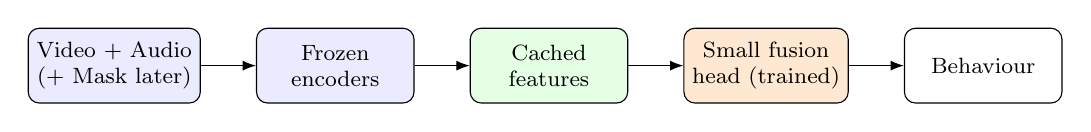
\begin{tikzpicture}[>=Latex,
    box/.style={draw, rounded corners, align=center, minimum width=2cm,
                minimum height=0.95cm, font=\footnotesize, inner sep=3pt}]
    \node[box, fill=blue!8]   (in)    {Video + Audio\\(+ Mask later)};
    \node[box, fill=blue!8, right=0.7cm of in]    (enc)  {Frozen\\encoders};
    \node[box, fill=green!10, right=0.7cm of enc] (cache){Cached\\features};
    \node[box, fill=orange!18, right=0.7cm of cache](head){Small fusion\\head (trained)};
    \node[box, right=0.7cm of head] (out) {Behaviour};
    \draw[->] (in)--(enc); \draw[->] (enc)--(cache);
    \draw[->] (cache)--(head); \draw[->] (head)--(out);
  \end{tikzpicture}
  \end{center}
  \vfill
  \begin{itemize}
    \item Cheap to run; the same cached features serve every experiment.
    \item Capacity stays identical across modalities, so any gain reflects
          \emph{information}, not parameters.
    \item The mask stream is \textbf{droppable at test time} (modality dropout).
  \end{itemize}
\end{frame}

% ---------------------------------------------------------------------
\begin{frame}{The frozen building blocks (we \emph{don't} train these)}
  Off-the-shelf \textbf{pretrained} models, run once and cached --- never updated:
  \vfill
  \begin{center}\footnotesize
  \begin{tabular}{@{}llp{4.8cm}@{}}
    \toprule
    Modality & Pretrained model & Input $\rightarrow$ output \\
    \midrule
    Video & VideoMAE (Kinetics) & 16 frames $\rightarrow$ 768-d vector \\
    Audio & AST (AudioSet)      & wav $\rightarrow$ spectrogram $\rightarrow$ 768-d vector \\
    Shape & SAM\,2 $+$ shape descriptors & frame $+$ animal box $\rightarrow$ \emph{mask} $\rightarrow$ shape numbers \\
    \bottomrule
  \end{tabular}
  \end{center}
  \vfill
  \begin{itemize}
    \item \textbf{SAM\,2 is the odd one out:} a \emph{segmentation} model --- it outputs a
          \emph{mask}, not an embedding. We turn the mask into shape numbers and a
          \emph{tiny} temporal encoder summarises them over time.
    \item \textbf{Only the fusion head is trained} --- the three big models never learn
          anything in this project.
  \end{itemize}
\end{frame}

% ---------------------------------------------------------------------
\begin{frame}{Progress so far}
  \begin{itemize}
    \item \textbf{Dataset secured \& verified} --- MammAlps Benchmark I; splits confirmed
          (train 4205 / val 686 / test 1244 / total 6135), matching the paper.
    \item \textbf{Scoring contract locked} --- a dummy-prediction file passes the official
          evaluator's exact format check (the 1244-clip assertion).
    \item \textbf{Frozen encoder path working} --- a real clip runs through VideoMAE and the
          audio encoder to give 768-d embeddings on the laptop GPU.
    \item \textbf{Reproducible codebase} --- config-driven, tested, on GitHub
          (\texttt{mambr}); proposal and write-up scaffolding in place.
  \end{itemize}
  \vfill
  \begin{center}
    \emph{Foundations are in place; no behaviour model trained yet --- that is next.}
  \end{center}
\end{frame}

% ---------------------------------------------------------------------
\begin{frame}{Plan / next steps}
  \begin{enumerate}
    \item Cache features for all 6{,}135 clips on a Kaggle GPU (run once).
    \item Reproduce the \textbf{video} and \textbf{video+audio} baseline
          (target $\approx$\,0.45 / 0.47 class-average mAP).
    \item Add the \textbf{SAM\,2 shape} modality and run the ablation:\\
          video $\rightarrow$ +mask $\rightarrow$ +audio $\rightarrow$ +audio+mask.
    \item \textbf{Per-behaviour analysis} (chasing, courtship) and a background-shift
          robustness test.
  \end{enumerate}
  \vfill
  \begin{block}{Bar for success}
    A clean baseline, then: does shape help \emph{where background did not}?
    Even a clean negative result is publishable.
  \end{block}
\end{frame}

% ---------------------------------------------------------------------
\begin{frame}{Discussion}
  \begin{itemize}
    \item Does the scope (single-animal MammAlps clips + a controlled multi-animal set for
          contact behaviours) look right?
    \item Any preference on the exact frozen encoders / compute?
    \item Happy to share the short proposal and the repository.
  \end{itemize}
  \vfill
  \begin{center}
    \Large Thank you --- questions \& feedback welcome!
  \end{center}
\end{frame}

\end{document}
